\section{実験の目的}
本研究では,RW によるグラフ取得をしながらノード ID を再配置する手法として,Sequential と DBG-EE を提案した.
そこで,実世界グラフのデータセットを用いて Sequential 及び DBG-EE を適用した場合の効果を実験から明らかにする.
具体的には,グラフ取得の完了を待たないことによる空間・時間コストの変化及びグラフ演算時間の減少率に着目する.
\section{実験概要}
\subsection{データセット}
実世界グラフのデータセットとして,スタンフォード大学が提供するグラフデータセットライブラリ SNAP \cite{snapnets} 内の 
Pokec Social Network \cite{takac2012data} を使用した.
表 \ref{dataset} に Pokec Social Network のグラフ情報を示す.
90 \% 有効直径とはノード間の最短距離の分布において 90 パーセンタイルに相当する値であり,
任意のノード間で最短距離が 5.2 以下となる確率が 90 \% であることを意味している.
\begin{table}[t]
  \begin{center}
    \caption{Pokec Social Network の概要}
    \begin{tabular}{cc} \toprule
      ノード数 & 1,632,803 \\
      エッジ数 & 30,622,564 \\
      90 \% 有効直径 & 5.2 \\ \bottomrule
    \end{tabular}
    \label{dataset}
  \end{center}
\end{table}

\subsection{パラメータの決定方法}
まず,RW 回数 N の決定方法について述べる.
表 \ref{rw_graph} で示すように,全体グラフのエッジ数に対する取得グラフのエッジ数は N = 100 万 のとき約 5 \%, N = 300 万 のとき約 10 \% となることが
実験的に明らかになった.
5 \% - 10 \% 程度のエッジを取得するという状況は全体グラフの一部を取得するという前提に矛盾しないと
判断し,N = 100 万,300 万をパラメータとして採用した.

次に,始点へ戻る確率 α の決定方法について述べる.
一般に,RW において始点に戻るまでの平均経路長は 1/α であることが知られている.
この平均経路長を 90 \% 有効直径と同程度に設定することで,始点の周辺グラフだけを密に取得し,
全体グラフの構造が失われる状況を回避できる.
表 \ref{dataset} で示すように,Pokec Social Network の 90 \% 有効直径は約 5 なので,α = 0.2 を
採用することで平均経路長と 90 \% 有効直径を同程度に設定した. 

表 \ref{parameter} に全パラメータの値を示す.
M は DBG-EE における再配置実行間隔に対応している.
なお,RW の開始点としてグラフ上の最高次数ノードを採用した.
\begin{table}[t]
  \begin{center}
    \caption{RW 回数と取得したエッジ数の割合の関係}
    \begin{tabular}{cccc} \toprule
      RW 回数 & ノード数 & エッジ数 & 取得したエッジ数の割合 \\ \hline
      100 万回 & 435,934 & 1,411,607 & 4.61 \% \\
      300 万回 & 686,506 & 3,409,700 & 11.3 \% \\ \bottomrule
    \end{tabular}
    \label{rw_graph}
  \end{center}
\end{table}
\begin{table}[t]
  \begin{center}
    \caption{各パラメータの値}
    \begin{tabular}{cc} \toprule
      N & 100 万, 300 万 \\
      M & 1 万,10 万 \\
      α & 0.2 \\ \bottomrule
    \end{tabular}
    \label{parameter}
  \end{center}
\end{table}


\subsection{対象とするグラフ演算}
RW で取得したグラフに対して PageRank (PR) と Personalized PageRank (PPR) を実行した.
なお,PR の計算には Ligra \cite{shun2013ligra} を,PPR の計算には FORA \cite{wang2017fora} を使用した.

\section{評価概要}
評価項目は以下の 3 点である.
\begin{itemize}
  \item ID 再配置を実行するためのメモリ使用量
  \item グラフ取得開始から演算終了までの合計時間 
  \item グラフ演算のみに要する時間
\end{itemize}
提案手法である Sequential,DBG-EE の比較対象は ID 再配置を実行しない Original,既存手法の DBG である.
なお,評価環境は表 \ref{eval_env} に示す通りである.
\begin{table}[t]
  \begin{center}
    \caption{評価環境}
    \begin{tabular}{cc} \toprule
      OS & Ubuntu Server 16.04 LTS \\
      CPU & Intel(R) Xeon(R) E5-2680 v3 @ 2.50 GHz \\
      RAM & 32 GB \\
      L1 キャッシュ & 32 KB  \\
      L2 キャッシュ & 256 KB \\
      L3 キャッシュ & 32 MB \\ \bottomrule 
    \end{tabular}
    \label{eval_env}
  \end{center}
\end{table}

\section{ID 再配置を実行するためのメモリ使用量}
まず,ID 再配置を実行するためのメモリ使用量を DBG に対する割合として測定した.
N = 100 万での結果を図 \ref{memory_usage_1000000} に,
N = 300 万での結果を図 \ref{memory_usage_3000000} に示す. 
Sequential は N = 100 万でメモリ使用量が 40.0 \% 減少,N = 300 万で 41.9 \% 減少と両方の場合でメモリ使用量の減少率が最大となった.
DBG-EE では M = 10,000 の場合 N = 100 万で 29.5 \% 減少,N = 300 万で 35.4 \% 減少し,
M = 100,000 の場合 N = 100 万で 16.5 \% 減少,N = 300 万で 26.8 \% 減少した.
これらの結果から,Sequential,DBG-EE はグラフ取得の完了を待たないことで空間コストの削減を達成できていることが明らかとなった.
しかし,DBG-EE では M の値が大きいほど取得途中で保持しなければならないグラフ構造が巨大化するため,
M = 100,000 の場合で M = 10,000 の場合より減少率が低下した.
また,N = 100 万より N = 300 万の方が減少率が大きいことから,
取得するグラフのサイズが大きいほど Sequential, DBG-EE の効果が大きいことが明らかとなった.
\begin{figure}[t]
  \centering
  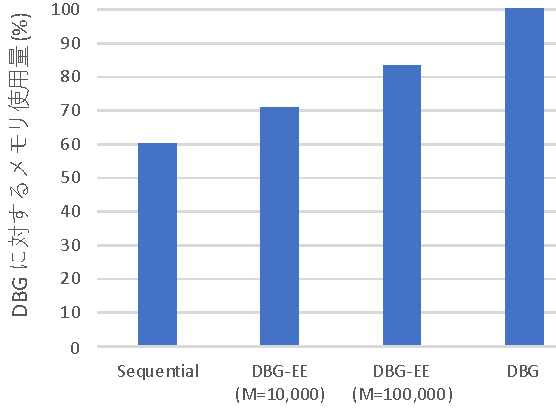
\includegraphics[width=0.8\linewidth]{./figure/memory_usage_10000.pdf}
  \caption{N = 100 万の場合における DBG に対するメモリ使用量}
  \label{memory_usage_1000000}
\end{figure}

\begin{figure}[t]
  \centering
  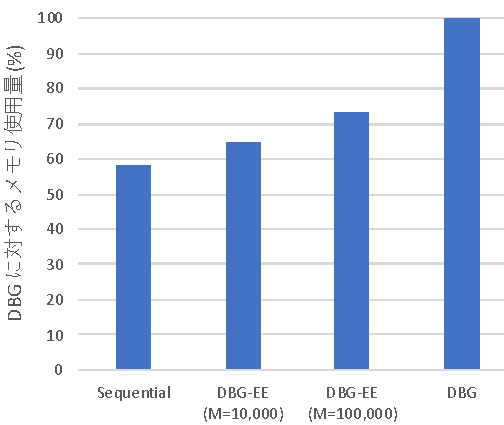
\includegraphics[width=0.8\linewidth]{./figure/memory_usage_3000000.pdf}
  \caption{N = 300 万の場合における DBG に対するメモリ使用量}
  \label{memory_usage_3000000}
\end{figure}

\section{グラフ取得開始から演算終了までの合計時間}
\label{total_time}
次に,グラフ取得を開始してから PR 演算が終了するまでの合計時間を計測した.
N = 100 万での結果を図 \ref{total_time_1000000} に,
N = 300 万での結果を図 \ref{total_time_3000000} に示す.

まず,図\ref{total_time_1000000} で示すように,N = 100 万のとき Original と比べて合計時間が M = 10,000 の場合の DBG-EE で 28.8 \% 減少,M = 100,000 の場合の DBG-EE で 30.7 \% 減少, 
Sequential で 25.5 \% 減少した.
また,DBG と比べて M = 10,000 の場合の DBG-EE で 7.8 \% 減少,M = 100,000 の場合で 10.3 \% 減少, 
Sequential で 4.5 \% 減少し,全ての場合で DBG より合計時間が減少した.
これらの結果から N = 100 万のとき Sequential,DBG-EE はグラフ取得の完了を待たないことで時間コストの削減を達成できていることが明らかとなった.
%最も時間コストが削減されたのは M = 100,000 の場合の DBG-EE で DBG と比べて合計時間が 11 \% 短縮している.
また,図\ref{total_time_3000000} で示すように N = 300 万のとき Original と比べて M = 10,000 の場合の DBG-EE で 14.5 \% 減少,M = 100,000 の場合で 16.5 \% 減少, 
Sequential で 9.9 \% 減少し,全ての場合で Orginal より合計時間が減少した.
一方で,DBG と比べて M = 10,000 の場合の DBG-EE で 4.1 \% 減少,M = 100,000 の場合の DBG-EE で 6.3 \% 減少,
Sequential で 1.1 \% 増加と,Sequential で DBG より合計時間が増加した.

Sequential で合計時間が増加した要因として 2 点考えられる.
まず DBG や DBG-EE と比べてグラフ演算に要する時間が長い点が挙げられる.これは\ref{algo_time} 節で詳しく述べる.
次に, RW によるグラフ取得の時間コストが大きい点が挙げられる.
図\ref{sequential} で示すように,Sequential は RW で 1 ノード移動する度に移動先のノードが再配置済みかを確認する.
この確認に伴い発生する時間コストが図\ref{total_time_3000000} における Original の RW 時間と Sequential の RW 時間の差に現れている.
DBG は取得完了後の再配置に伴い時間コストが発生するが,RW によるグラフ取得自体にかかる時間コストは Original と等しい.
そのため,Sequential で再配置に伴う時間コスト減少の効果が弱まり,DBG より合計時間が増加した.
\begin{figure}[t]
  \centering
  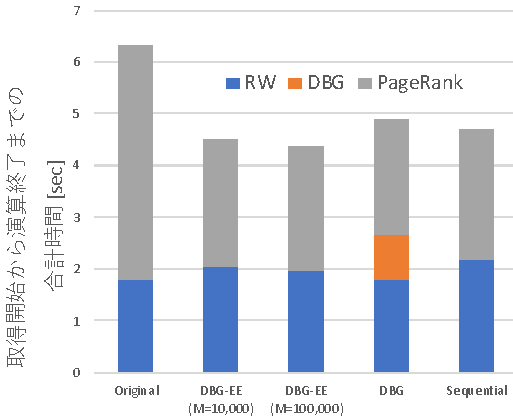
\includegraphics[width=0.8\linewidth]{./figure/total_time_1000000.pdf}
  \caption{N = 100 万の場合におけるグラフ取得と演算の合計時間}
  \label{total_time_1000000}
\end{figure}
\begin{figure}[t]
  \centering
  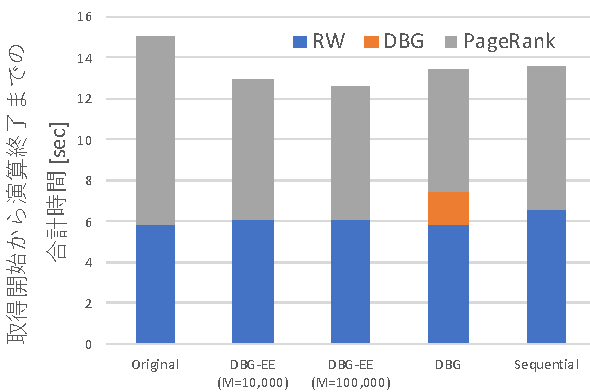
\includegraphics[width=0.8\linewidth]{./figure/total_time_3000000.pdf}
  \caption{N = 300 万の場合におけるグラフ取得と演算の合計時間}
  \label{total_time_3000000}
\end{figure}

\section{演算のみに要する時間}
\label{algo_time}
最後に,PR と PPR の演算のみに要する時間を測定した.
N = 100 万での結果を図 \ref{algo_time_1000000} に,
N = 300 万での結果を図 \ref{algo_time_3000000} に示す.
まず,図\ref{algo_time_1000000} で示すように,N = 100 万のとき Original と比べて PR 演算時間が M = 10,000 の場合の DBG-EE で 45.7 \% 減少,M = 100,000 の場合の DBG-EE で 46.8 \% 減少, 
Sequential で 44.4 \% 減少した. 
また,PPR 演算時間は Original と比べて M = 10,000 の場合の DBG-EE で 25.4 \% 減少,M = 100,000 の場合の DBG-EE で 27.6 \% 減少, 
Sequential で 40.6 \% 減少した.
さらに,図\ref{algo_time_3000000} で示すように,N = 300 万のとき Original と比べて PR 演算時間が M = 10,000 の場合の DBG-EE で 26.7 \% 減少,M = 100,000 の場合の DBG-EE で 29.3 \% 減少, 
Sequential で 24.4 \% 減少した.
また,PPR 演算時間は Original と比べて M = 10,000 の場合の DBG-EE で 16.0 \% 減少,M = 100,000 の場合の DBG-EE で 16.9 \% 減少, 
Sequential で 20.3 \% 減少した.
これらの結果から,Sequential,DBG-EE ともに 全ての場合で Sequential より演算時間が減少しており,
PR では DBG-EE の方が減少率が大きく,PPR では Sequential の方が減少率が大きいことが明らかとなった.
なお,N が大きいほど減少率が低下することが明らかとなった.
これは,より多くのグラフ構造を取得するほど Original が全体グラフに近づき,ID の連続性が向上するからだと考えられる.

一方で,DBG と比べて N = 100 万のとき PR 演算時間は M = 10,000 の場合の DBG-EE で 11.4 \% 増加,M = 100,000 の場合の DBG-EE で 9.1 \% 増加, 
Sequential で 14.1 \% 増加した.
また,PPR 演算時間は DBG と比べて M = 10,000 の場合の DBG-EE で 7.3 \% 増加,M = 100,000 の場合の DBG-EE で 4.1 \% 増加, 
Sequential で 14.5 \% 減少した.
さらに,N = 300 万のとき PR 演算時間は M = 10,000 の場合の DBG-EE で 14.1 \% 増加,M = 100,000 の場合の DBG-EE で 10.1 \% 増加, 
Sequential で 17.6 \% 増加した.
また,PPR 演算時間は M = 10,000 の場合の DBG-EE で 3.0 \% 増加,M = 100,000 の場合の DBG-EE で 2.0 \% 増加, 
Sequential で 2.3 \% 減少した.

DBG ではグラフの取得が完了してから再配置するため ID の連続性と演算時の局所性の双方が考慮されている.
そのため,一般に DBG-EE や Sequential の方が演算に時間がかかるが,\ref{total_time} 節で述べたように,
取得開始からの合計時間が DBG を下回ることで全体の時間コスト削減を達成している.
なお,PPR 演算時間において Sequential が DBG を下回っている.
Sequential と DBG はどちらも ID の連続性が保証されているため,アクセス局所性によって演算時間に差が発生したと考えられる.
Sequential では 部分的に近接構造によるアクセス局所性を考慮した ID 再配置が実現されており,PPR 演算においては Sequential の近接構造によるアクセス局所性が有利に働いたと考えられる.
これらの考察から,対象とするアルゴリズム毎にどのようなアクセス局所性を考慮すべきか明らかにすることは今後の課題である.

\begin{figure}[t]
  \centering
  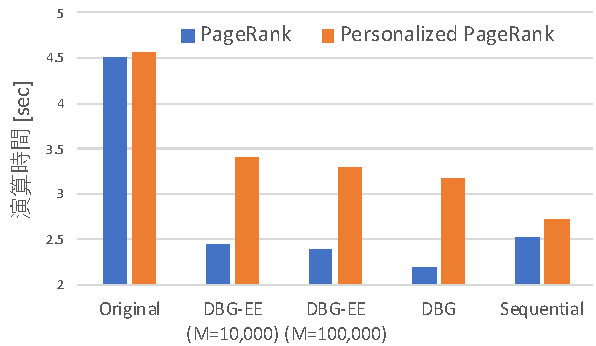
\includegraphics[width=0.8\linewidth]{./figure/algo_time_1000000.pdf}
  \caption{N = 100 万の場合における PR, PPR 演算時間}
  \label{algo_time_1000000}
\end{figure}
\begin{figure}[t]
  \centering
  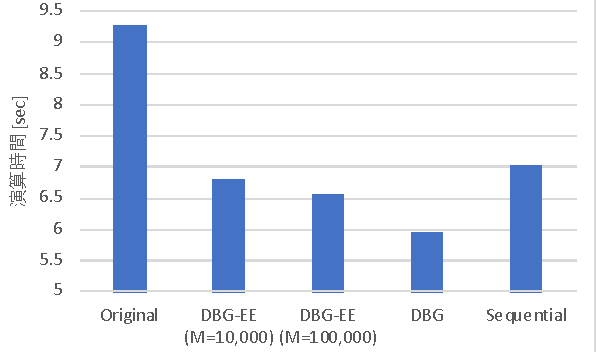
\includegraphics[width=0.8\linewidth]{./figure/algo_time_3000000.pdf}
  \caption{N = 300 万の場合における PR, PPR 演算時間}
  \label{algo_time_3000000}
\end{figure}